% flashcards-title: Two column setups of the same decimal addition
% flashcards-desc: Two column-form setups of the decimal addition four point six plus zero point eight five, labeled A and B. In layout A the final digits of the two numbers are flush right, so the six sits above the five. In layout B the decimal points sit directly above one another, so the six sits above the eight. Each layout shows a plus sign beside the lower number and a horizontal answer line below it.
\documentclass[tikz]{standalone}
\usetikzlibrary{arrows.meta,patterns}

\definecolor{qraNavy}{HTML}{17324D}
\definecolor{qraBlue}{HTML}{2B6CB0}
\definecolor{qraGold}{HTML}{B7791F}
\definecolor{qraPale}{HTML}{EAF2F8}
\definecolor{qraGray}{HTML}{5C6773}

\tikzset{
  qra axis/.style={draw=qraNavy, line width=1.2pt},
  qra tick/.style={draw=qraNavy, line width=1pt},
  qra guide/.style={draw=qraGray, densely dashed, line width=0.8pt},
  qra counter/.style={circle, draw=qraNavy, fill=qraPale, line width=0.9pt, minimum size=7mm, inner sep=0pt},
  qra label/.style={font=\sffamily\bfseries, text=qraNavy},
  qra small label/.style={font=\sffamily, text=qraNavy},
}

\begin{document}
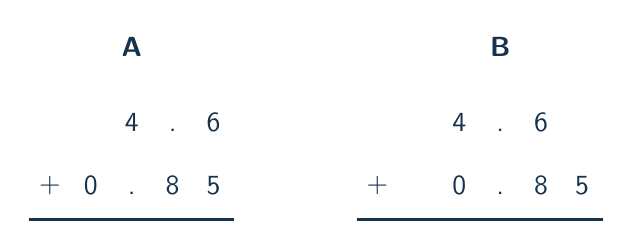
\begin{tikzpicture}[x=0.52cm, y=0.8cm]
  % ----- Layout A: last digits flush right -----
  \node[qra label] at (2.0,2.2) {A};
  % Row 1:      4 . 6   (right-aligned against column 4)
  \node[qra small label] at (2,1) {4};
  \node[qra small label] at (3,1) {.\vphantom{0}};
  \node[qra small label] at (4,1) {6};
  % Row 2:  + 0 . 8 5
  \node[qra small label] at (0,0) {$+$};
  \node[qra small label] at (1,0) {0};
  \node[qra small label] at (2,0) {.\vphantom{0}};
  \node[qra small label] at (3,0) {8};
  \node[qra small label] at (4,0) {5};
  \draw[qra axis] (-0.5,-0.55) -- (4.5,-0.55);
  % ----- Layout B: decimal points aligned -----
  \node[qra label] at (11.0,2.2) {B};
  % Row 1:      4 . 6
  \node[qra small label] at (10,1) {4};
  \node[qra small label] at (11,1) {.\vphantom{0}};
  \node[qra small label] at (12,1) {6};
  % Row 2:  + 0 . 8 5
  \node[qra small label] at (8,0) {$+$};
  \node[qra small label] at (10,0) {0};
  \node[qra small label] at (11,0) {.\vphantom{0}};
  \node[qra small label] at (12,0) {8};
  \node[qra small label] at (13,0) {5};
  \draw[qra axis] (7.5,-0.55) -- (13.5,-0.55);
\end{tikzpicture}
\end{document}
